% Generated 2020-10-22 16:25:25 +0530
\subsection{Specifications} \label{sec:Specifications}


\begin{figure}[ht]
  \centering
    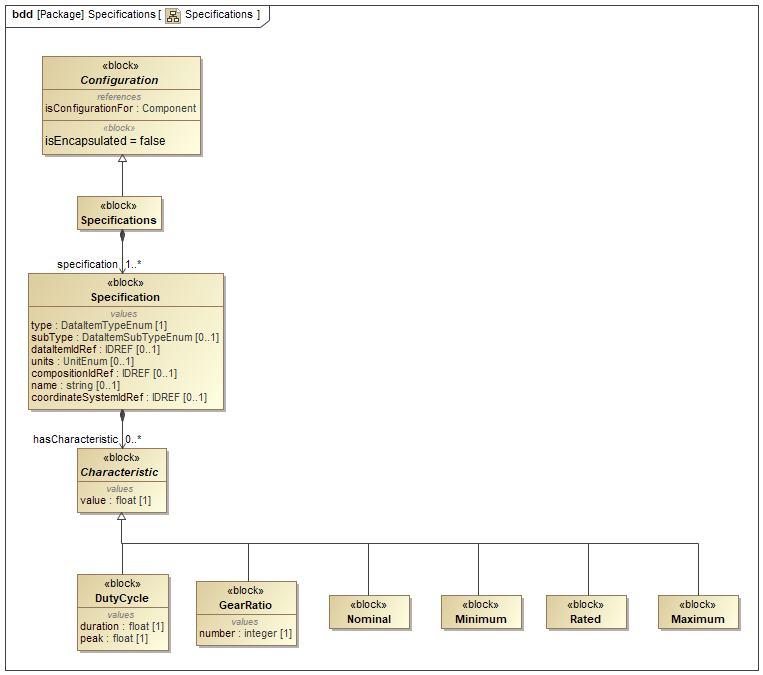
\includegraphics[width=1.0\textwidth]{figures/Specifications.png}
  \caption{Specifications Diagram}
  \label{fig:Specifications}
\end{figure}

\FloatBarrier



\subsubsection{Characteristic}
\label{sec:Characteristic}






\paragraph{Attributes of Characteristic}\mbox{}
\label{sec:Attributes of Characteristic}

\tbl{Attributes of Characteristic} lists the attributes of \texttt{Characteristic}.

\begin{table}[ht]
\centering 
  \caption{Attributes of Characteristic}
  \label{table:Attributes of Characteristic}
\tabulinesep=3pt
\begin{tabu} to 6in {|l|l|l|} \everyrow{\hline}
\hline
\rowfont\bfseries {Attribute} & {Type} & {Multiplicity} \\
\tabucline[1.5pt]{}
\property{value}[Characteristic] & \texttt{float} & 1 \\
\end{tabu}
\end{table}
\FloatBarrier


Descriptions for attributes of \block{Characteristic}:

\begin{itemize}

\item \property{value}[Characteristic] : 
\end{itemize}

\subsubsection{Rated}
\label{sec:Rated}






\subsubsection{Minimum}
\label{sec:Minimum}



A numeric lower limit constraint.


\subsubsection{Maximum}
\label{sec:Maximum}



A numeric upper limit constraint.


\subsubsection{GearRatio}
\label{sec:GearRatio}






\paragraph{Attributes of GearRatio}\mbox{}
\label{sec:Attributes of GearRatio}

\tbl{Attributes of GearRatio} lists the attributes of \texttt{GearRatio}.

\begin{table}[ht]
\centering 
  \caption{Attributes of GearRatio}
  \label{table:Attributes of GearRatio}
\tabulinesep=3pt
\begin{tabu} to 6in {|l|l|l|} \everyrow{\hline}
\hline
\rowfont\bfseries {Attribute} & {Type} & {Multiplicity} \\
\tabucline[1.5pt]{}
\property{number}[GearRatio] & \texttt{integer} & 1 \\
\end{tabu}
\end{table}
\FloatBarrier


Descriptions for attributes of \block{GearRatio}:

\begin{itemize}

\item \property{number}[GearRatio] : 
\end{itemize}

\subsubsection{Nominal}
\label{sec:Nominal}



The numeric target or expected value.


\subsubsection{DutyCycle}
\label{sec:DutyCycle}






\paragraph{Attributes of DutyCycle}\mbox{}
\label{sec:Attributes of DutyCycle}

\tbl{Attributes of DutyCycle} lists the attributes of \texttt{DutyCycle}.

\begin{table}[ht]
\centering 
  \caption{Attributes of DutyCycle}
  \label{table:Attributes of DutyCycle}
\tabulinesep=3pt
\begin{tabu} to 6in {|l|l|l|} \everyrow{\hline}
\hline
\rowfont\bfseries {Attribute} & {Type} & {Multiplicity} \\
\tabucline[1.5pt]{}
\property{duration}[DutyCycle] & \texttt{float} & 1 \\
\property{peak}[DutyCycle] & \texttt{float} & 1 \\
\end{tabu}
\end{table}
\FloatBarrier


Descriptions for attributes of \block{DutyCycle}:

\begin{itemize}

\item \property{duration}[DutyCycle] : 

\item \property{peak}[DutyCycle] : 
\end{itemize}

\subsubsection{Specification}
\label{sec:Specification}



\block{Specification} elements define information describing the design characteristics for a piece of equipment.



\paragraph{Attributes of Specification}\mbox{}
\label{sec:Attributes of Specification}

\tbl{Attributes of Specification} lists the attributes of \texttt{Specification}.

\begin{table}[ht]
\centering 
  \caption{Attributes of Specification}
  \label{table:Attributes of Specification}
\tabulinesep=3pt
\begin{tabu} to 6in {|l|l|l|} \everyrow{\hline}
\hline
\rowfont\bfseries {Attribute} & {Type} & {Multiplicity} \\
\tabucline[1.5pt]{}
\property{type}[Specification] & \texttt{DataItemTypeEnum} & 1 \\
\property{subType}[Specification] & \texttt{DataItemSubTypeEnum} & 0..1 \\
\property{dataItemIdRef}[Specification] & \texttt{IDREF} & 0..1 \\
\property{units}[Specification] & \texttt{UnitEnum} & 0..1 \\
\property{compositionIdRef}[Specification] & \texttt{IDREF} & 0..1 \\
\property{name}[Specification] & \texttt{string} & 0..1 \\
\property{coordinateSystemIdRef}[Specification] & \texttt{IDREF} & 0..1 \\
\end{tabu}
\end{table}
\FloatBarrier


Descriptions for attributes of \block{Specification}:

\begin{itemize}

\item \property{type}[Specification] : Same as \block{DataItem} type. See \sect{DataItem Types}.

\item \property{subType}[Specification] : Same as \block{DataItem} subtypes. See \sect{DataItem SubTypes}.

\item \property{dataItemIdRef}[Specification] : A reference to the \property{id} attribute of the \block{DataItem} associated with this element.

\item \property{units}[Specification] : Same as \block{DataItem} units. See \sect{DataItem}.

\item \property{compositionIdRef}[Specification] : A reference to the \property{id} attribute of the \block{Composition} associated with this element.

\item \property{name}[Specification] : The \property{name} provides additional meaning and differentiates between \block{Specifications}.

\item \property{coordinateSystemIdRef}[Specification] : References the \block{CoordinateSystem} for geometric \block{Specification} elements.
\end{itemize}

\paragraph{Elements of Specification}\mbox{}
\label{sec:Elements of Specification}

\tbl{Elements of Specification} lists the elements of \texttt{Specification}.

\begin{table}[ht]
\centering 
  \caption{Elements of Specification}
  \label{table:Elements of Specification}
\tabulinesep=3pt
\begin{tabu} to 6in {|l|l|l|} \everyrow{\hline}
\hline
\rowfont\bfseries {Element Name} & {Type} & {Multiplicity} \\
\tabucline[1.5pt]{}
\block{Characteristic} & \texttt{Characteristic} & 0..* \\
\end{tabu}
\end{table}
\FloatBarrier


Descriptions for elements of \block{Specification}:

\begin{itemize}
\item \block{Characteristic} : 
\end{itemize}

\subsubsection{Specifications}
\label{sec:Specifications}



\block{Specifications} \glspl{organize} \block{Specification} elements for a \block{Component}.


\paragraph{Elements of Specifications}\mbox{}
\label{sec:Elements of Specifications}

\tbl{Elements of Specifications} lists the elements of \texttt{Specifications}.

\begin{table}[ht]
\centering 
  \caption{Elements of Specifications}
  \label{table:Elements of Specifications}
\tabulinesep=3pt
\begin{tabu} to 6in {|l|l|l|} \everyrow{\hline}
\hline
\rowfont\bfseries {Element Name} & {Type} & {Multiplicity} \\
\tabucline[1.5pt]{}
\block{Specification} & \texttt{Specification} & 1..* \\
\end{tabu}
\end{table}
\FloatBarrier


Descriptions for elements of \block{Specifications}:

\begin{itemize}
\item \block{Specification} : \block{Specification} elements define information describing the design characteristics for a piece of equipment.

\end{itemize}
